\section{O papel do analisador léxico}

\begin{frame}[fragile]{Analisador léxico}

    \begin{itemize}
        \item A análise léxica é a primeira fase de um compilador
        \pause

        \item Um analisador léxico deve ser os caracteres da entrada e produzir uma sequência de tokens, os quais serão usados pelo \textit{parser} durante a
            análise sintática
        \pause

        \item Uma forma de se construir um analisador léxico é escrever um diagrama que ilustre a estrutura dos tokens da linguagem fonte e o traduzir manualmente
            em um programa que os identifique
        \pause

        \item As técnicas de construção de um analisador léxico podem ser utilizadas em outras áreas
        \pause

        \item Como o analisador léxico é responsável pela leitura do programa fonte, ele pode também realizar tarefas secundárias a nível de interface com
            o usuário, como a remoção e espaços e comentários, por exemplo
    \end{itemize}

\end{frame}

\begin{frame}[fragile]{Interação entre o analisador léxico e o {\it parser}}

    \begin{figure}
        \centering 

        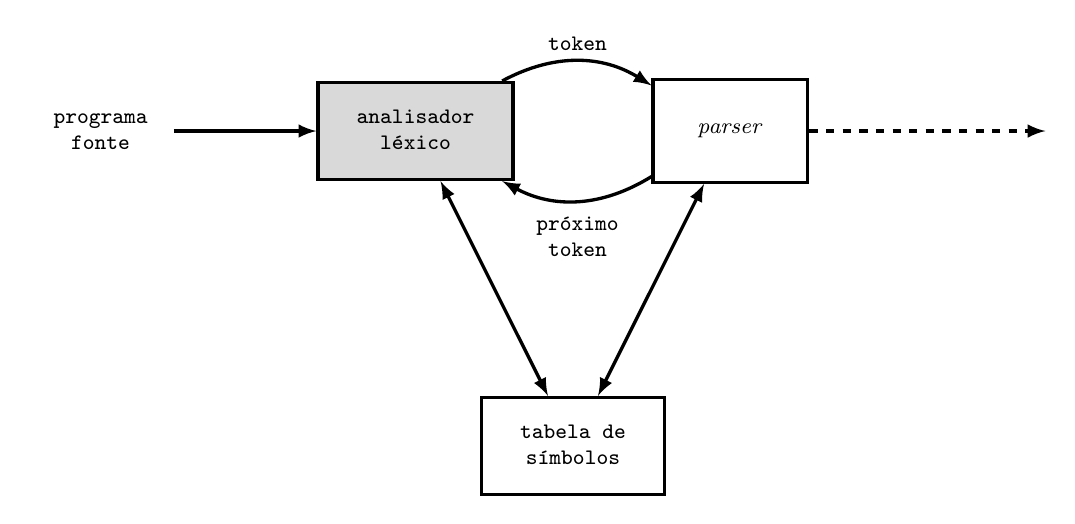
\begin{tikzpicture}
            \node (A) at (0, 6) {\footnotesize \texttt{\begin{tabular}{c}programa\\ fonte\end{tabular}} };
            \node[draw,very thick,inner sep=8pt,fill=gray!30] (B) at (4, 6) {\footnotesize \texttt{\begin{tabular}{c}analisador\\ léxico\end{tabular}} };
            \node[draw,very thick,inner sep=16pt] (C) at (8, 6) {\footnotesize \textit{parser} };
            \node[draw,very thick,inner sep=8pt] (D) at (6, 2) {\footnotesize \texttt{\begin{tabular}{c}tabela de\\ símbolos\end{tabular}} };

            \draw[very thick,-latex] (A) to (B);
            \draw[very thick,-latex] (B) to [bend left] node[above] {\footnotesize \texttt{token}} (C);
            \draw[very thick,-latex] (C) to [bend left] node[below] {\footnotesize \texttt{\begin{tabular}{c}próximo\\ token\end{tabular}}} (B);
            \draw[very thick,-latex,dashed] (C) to (12, 6);
            \draw[very thick,latex-latex] (B) to (D);
            \draw[very thick,latex-latex] (C) to (D);
        \end{tikzpicture}
    \end{figure}

\end{frame}

\begin{frame}[fragile]{Separação entre a análise léxica e a análise gramatical}

    Há quatro principais motivos para se separar a análise léxica da análise gramatical (\textit{parsing}):
    \pause
    \begin{enumerate}
        \item A separação entre estas duas fases pode simplificar uma das duas (ou ambas)
        \pause

        \item A eficiência do compilador é melhorada, uma vez que a separação permite o uso de técnicas especializadas, como buferização, para melhorar o 
            desempenho da leitura da entrada e extração de tokens
        \pause

        \item A separação permite uma melhor portabilidade do compilador, uma vez que diferenças entre a captura da entrada e codificação de caracteres,
        em diferentes plataformas, podem ser tratadas de forma isolada na análise léxica
        \pause

        \item A separação entre as fases permite a criação de ferramentas especilizadas para a automação da construção de analisadores léxicos e de \textit{parsers}
    \end{enumerate}

\end{frame}

\begin{frame}[fragile]{Tokens, padrões e lexemas}

    \begin{itemize}
        \item Tokens, padrões e lexemas são conceitos correlacionados e onipresentes na análise léxica
        \pause

        \item Token é um símbolo terminal da gramática da linguagem fonte (em geral, grafados em negrito)
        \pause

        \item Nas maioria das linguagens de programação, são tokens: palavras-chave, operadores, identificadores, constantes, pontuações, etc
        \pause

        \item Um lexema é um conjunto de caracteres que é reconhecido como um token
        \pause

        \item Um mesmo token pode ser representado por lexemas distintos (por exemplo, 1 e 42 são lexemas distintos para o token \code{cpp}{NUM})
        \pause

        \item Um padrão descreve o conjunto de lexemas que podem representar um token em particular
    \end{itemize}

\end{frame}

\begin{frame}[fragile]{Atributos para tokens}

    \begin{itemize}
        \item Quando dois ou mais lexemas estão associados a um mesmo token, o analisador léxico deve prover informações adicionais para as fases subsequentes,
            para que elas possam distinguí-los
        \pause

        \item Estas informações são os atributos do token
        \pause

        \item Deste modo, o analisador léxico deve identificar os tokens e seus respectivos atributos, caso existam
        \pause

        \item Os tokens influenciam as decisões da análise gramatical
        \pause

        \item Os atributos influenciam a tradução dos tokens
        \pause

        \item Em tokens numéricos, o valor do número representado pelo lexema pode ser o atributo token
        \pause

        \item No caso de identificadores, o próprio lexema pode ser o atributo do token
    \end{itemize}

\end{frame}

\begin{frame}[fragile]{Erros léxicos}

    \begin{itemize}
        \item Determinados erros não podem ser detectados em nível léxico
        \pause

        \item Por exemplo, na expressão em C++
            \inputsyntax{cpp}{codes/if.cpp}
        o analisador léxico identificaria \code{cpp}{fi} como um identificador válido, e só na análise gramatical é que seria detectado o erro de digitação da
        palavra-chave \code{cpp}{if}
        \pause

        \item Os erros léxicos mais comuns são aqueles onde o analisador léxico não consegue associar o prefixo lido a nenhum dos padrões associados aos tokens
        da linguagem
        \pause

        \item Neste ponto, o analisador léxico pode abordar a leitura, emitindo uma mensagem de erro
        \pause

        \item Outra alternativa é tentar tratar o erro de alguma maneira
    \end{itemize}

\end{frame}

\begin{frame}[fragile]{Ações de recuperação de erros}

    Há quatro ações que configuram tentativas de recuperação de erros léxicos:
    \pause
    \begin{itemize}
        \item remover um caractere estranho da entrada
        \pause

        \item inserir um caractere ausente
        \pause

        \item substituir um dos caracteres incorretos por um caractere correto
        \pause

        \item transpor dois caracteres adjacentes
    \end{itemize}
    \pause

    \vspace{0.2in}

    Se uma ou mais ações conseguem tornar o prefixo em um token válido, o analisador podem indicar ao usuário a sequência de ações como sugestão de correção do
    programa fonte, ou mesmo prosseguir assumindo esta correção.
\end{frame}
